\documentclass{article}
\usepackage{graphicx}
\graphicspath{ {./images/} }
\setlength{\oddsidemargin}{0.25 in}
\setlength{\evensidemargin}{-0.25 in}
\setlength{\topmargin}{-0.6 in}
\setlength{\textwidth}{6.5 in}
\setlength{\textheight}{8.5 in}
\setlength{\headsep}{0.75 in}
\setlength{\parindent}{0 in}
\setlength{\parskip}{0.1 in}

% ===== PACKAGES =====
\usepackage{float}
\usepackage{amsmath,amssymb}
\usepackage{color}
\usepackage{subfigure}
\usepackage{mdframed}
\usepackage{changepage}
\usepackage{hyperref}
\newmdenv[
  topline=false,
  bottomline=false,
  skipabove=\topsep,
  skipbelow=\topsep
]{siderules}
\renewcommand{\abstractname}{}

% ===== VARIABLES =====
\def \R{\mathbb{R}}
\def \Pr{\mathbb{P}}
\def \D{{\rm D}}
\def \N{{\rm N}}
\def \xx{{\boldsymbol{\rm x}}}
\def \y{{\rm y}}




% ===== HEADER BOX =====
\newcommand{\lecture}[2]{
\pagestyle{myheadings}
\thispagestyle{plain}
\newpage
\noindent
\begin{center}
\rule{\textwidth}{1.6pt}\vspace*{-\baselineskip}\vspace*{2pt} % Thick horizontal line
\rule{\textwidth}{0.4pt}\\[1\baselineskip] % Thin horizontal line
\vbox{\vspace{2mm}
\hbox to 6.28in { {\bf CS 760: Machine Learning} \hfill Spring 2022 }
\vspace{4mm}
\hbox to 6.28in { {\Large \hfill #1  \hfill} }
\vspace{4mm}
\hbox to 6.28in { {\scshape Authors:}  #2 \hfill }}
\vspace{-2mm}
\rule{\textwidth}{0.4pt}\vspace*{-\baselineskip}\vspace{3.2pt} % Thin horizontal line
\rule{\textwidth}{1.6pt}\\[\baselineskip] % Thick horizontal line
\end{center}
\vspace*{4mm}
}



% =============== DOCUMENT ===============
\begin{document}
\lecture{Estimating adverse clinical outcomes and Biological Age using CT and Clinical Data}{Ganesh Cheerla(gcheerla), Harsh Sahu(hsahu), Hemalkumar Ratilal Patel(hrpatel5)}

\begin{center}
{\Large {\sf \underline{\textbf{DO NOT POLLUTE!}} AVOID PRINTING, OR PRINT 2-SIDED MULTIPAGE.}}
\end{center}


\begin{abstract}
We have a real dataset related to \textit{Opportunistic Cardiometabolic} Screening. The goal is to exploit the dataset collected for the mentioned reason to predict other clinical outcomes and measure biological age using incidental data that typically goes unused/underuse – this includes clinical data and Computerized Tomography (CT) data. For the context of this project, we have predicted death, diabetes and heart-attack and derived biological age.
\end{abstract}
\section{Introduction}

Our goals for this project are as below:
\begin{enumerate}
    \item Predict Clinical Outcomes using first only CT data, and then CT+Clinical data. Later we compare both outcomes to assess the effectiveness
    \begin{enumerate}
        \item Death
        \item Diabetes
        \item Heart-Attack
    \end{enumerate}
    \item Derive a patient's Biological Age
\end{enumerate}

For (1), we have split the data into train/test and considered relevant key clinical outcome column for that particular prediction, i.e., \textit{DEATH [d from CT]} for Death, \textit{Type 2 Diabetes DX Date [d from CT]} for Diabetes and \textit{MI DX Date [d from CT]} for Heart Attack.We have used 2 approaches for prediction, which we will describe in \textbf{Section 4}.

For (2), we have only considered CT data as an input features. CT data contains columns that are proven biological age markers and have been used widely in clinical research \cite{common_methods_of_biological_age_estimation} \cite{60_new_50} \cite{bio_using_PCA} already. We have formed train data using patient who have died, and rest are grouped into test data to calculate biological age. This is because we know for certainty that patient who died reached their biological limit. The exact methodology is explained in \textbf{Section 4}  


\section{Related Work}

There are studies that analyze a CT feature and examine its importance in predicting adversarial outcomes like death or critical illness. \cite{BMD}analyzes the impact of Bone Mineral Density of L1 vertebra. It mentions the values ranges of ${<}$ 100 to be osteopric which we try to validate in our experiments. Similarly, \cite{FAT} analyzes the impact of various fat measures like Visceral Adipose tissue area and Subcutaneous Adipose tissue area on health and metabolism of patients. We use these observations to get patterns from our data using different ratios like Total adipose tissue area/Body area, VAT/SAT. 
Aortic calcification is a measure of calcium deposit in heart's blood vessels. As per common medical knowledge, it is a best indicator of Heart Attack. We analyze the work about this feature \cite{AoCa}, and confirm through our experiments. Liver HU indicates the attenuation of liver fat. The lower this value, the higher the risk of fatal outcomes like death. This is anlyzed in \cite{Liver HU}

There have been clinical researches \cite{common_methods_of_biological_age_estimation} \cite{60_new_50} \cite{bio_using_PCA} to exploit biological health markers to effectively calculate biological age. All these studies have incorporated different techniques such as PCA, Linear Regression, multiple linear regression (MLR), Klemera and Doubal’s method (KDM) etc. All these studies collected data on healthy individuals periodically to assess how biological health markers get affected as the chronological age grows. They have considered them a baseline and then use that to calculate biological age of test samples.

However, we don't have the same type and amount of data as those studies. So we cannot use them as it is. However, the inspiration is that biological health markers are effective at measuring biological health.
\section{Dataset}
The dataset was made available by Perry Pickhardt (Department of Radiology, UW-Madison) who also provided guidance in supervising and evaluating this project. The dataset contains 3 set of columns.


\begin{itemize}
    \item Clinical Data
    \begin{itemize}
        \item Cols A-C: anonymized Case ID info
        \item Col D: Clinical F/U interval [days from CT]
        \item Cols E-J: pt BMI, sex, age (at time 0=CT date), smoking/drinking hx)
        \item Col K: FRS = Framingham Risk Score (multi variable 10-yr cardiovascular risk score)
        \item Cols L-M: FRAX = Fracture risk assessment score (multi-variable 10-yr risk for all and hip fx)
        \item Col N: Metabolic Syndrome (Y/N/blank=unknown) ? really more of an outcome
    \end{itemize}
    \item Clinical Outcomes
    \begin{itemize}
        \item Col P: Death
        \item Cols Q-V: Cardiovascular events w/ dates (CVD=stroke, Heart failure, MI=heart attack; any=positive)
        \item Col W-X: T2 Diabetes (if dx)
        \item Cols Y-AH: Pathologic/osteoporotic fracture w/ date (any=positive; femoral=hip fx)
        \item Cols AI-AJ: Alzheimer’s Dx
        \item Cols AK-AN: Cancer Dx’s
        \item Col N: Metabolic Syndrome; could be considered an outcome)
    \end{itemize}
    \item Computerized Tomography Data
    \begin{itemize}
        \item Col AP: Bone measure/BMD (L1 HU)
        \item Cols AQ-AU: Fat measures (total/visceral/subcutaneous; V/S ratio; all total body X-section)
        \item Cols AV-AX: Muscle measures (HU/Area/SMI)
        \item Col AY: Aortic Calcification (Ag)
        \item Col AZ: Liver fat (HU)

    \end{itemize}
\end{itemize}
\section{Approach}


\subsection{Packages}
We have extensively used python machine learning and data-science libraries throughout this project.

\begin{itemize}
    \item \textit{numpy} and \textit{pandas} are used to handle dataset and perform operations
    \item \textit{seaborn} and \textit{matplotlib} are used to visualize the dataset and output results
    \item \textit{sklearn} and \textit{xgboost} are used to run machine learning algorithms
\end{itemize}

\subsection{Data Cleaning and Pre-processing}

We have used data clipping to remove skewness in features. Columns \textit{AoCa Agatston} and \textit{Liver HU (Median)} are clipped at 99th percentile.

Moreover, the sparse nature of the dataset prompted us to fill \textit{NULL} values in CT data using the corresponding mean.

We have also used the iterative imputing strategy \cite{imputing} to fill null values in a few CT features. This type of imputing is useful when we know that a feature is dependent on other features. In this dataset, we have filled the NULL values in CT features using dependent clinical features. First, we get the correlation heatmap of all the features. Using this, we determine the features on which a CT feature is dependent. We will use these dependent features as related columns and apply \textit{sklearn.IterativeImpute}r. Under the hood, iterative imputer fits a linear regression model on non NULL values of related clinical features as 'features' and the CT feature as the 'target'. This ensures a more realistic NULL values as opposed to filling everything just by mean.
For example, we fill the NULL values in 'VAT/SAT ratio' using 'Muscle\_Area' and 'Sex' features.
We have also used correlation heatmap \ref{fig:heatmap} to drop features that are highly correlated and to add new features. We have removed TAT area and Total\_body\_area and added a new feature 'TAT area/Total\_body\_area'

\begin{figure}[h]
\centering
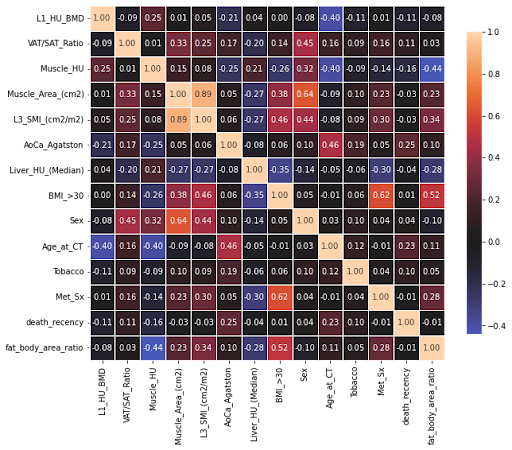
\includegraphics[width=0.8\textwidth]{images/heatmap.png}
\caption{Feature Heatmap}
\label{fig:heatmap}
\end{figure}

\subsection{Methodology - Predicting Death, Diabetes and Heart Attack}

For each 3 predictions, we first use only CT data, and then take the results again with CT + Clinical data. Our experiment involves running 3 algorithms, and comparing their corresponding RMSE(Root Mean Square Error)
\begin{enumerate}
    \item Linear Regression
    \item Support Vector Regressor
    \item XGBoost
\end{enumerate}

For each 3 predictions, we split the original dataset of size 9223 items in 80-20 train/test fashion. It includes both \textit{NULL} and \textit{NON-NULL} key columns. For example, for column \textit{DEATH [d from CT]} we have
\begin{itemize}
    \item Train Data - 7363, 6944 NULL, 419 NON-NULL
    \item Test Data - 1860, 1730 NULL, 130 NON-NULL
\end{itemize}

\subsubsection{Approach-1:}
We don't perform any other modification or data pre-processing in this approach.

For each 3 predictions, we perform the following operations:
\begin{enumerate}
    \item We train our model \textbf{only on NON-NULL training data} and test on NULL test data.
    \item We compare the distribution of values computed in the previous step with that of the NON-NULL test data
\end{enumerate}

\subsubsection{Approach-2: Recency}
In this approach, we introduced a new column \textit{recency}.
\[ death\_recency = 1 / DEATH[d\_from\_ CT]  \]
\[ diabetes\_recency = 1 /  DX\_Date[d\_from\_ CT]  \]
\[ heart\_attack\_recency = 1 / MI\_DX\_Date[d\_from\_ CT]  \]

This gives us the chance to fill all NULL values with zeros. However, it results in skewed data - Fig \ref{fig:recency_skewness_before_after_fix}. Hence, we transformed non-zero values (using Box-cox transform) to a more uniform distribution. Later, we sub-sampled zero samples to be equal to non-zero samples. This provides us with different training/test number of samples than the original. For example, for \textit{death\_recency} we got 838 training samples and 1860 test samples.

\begin{figure}[H]
	\def\imgwidth{0.5\linewidth}
% 	\setlength\tabcolsep{2pt}
	\centering
	\begin{tabular}{cc}
		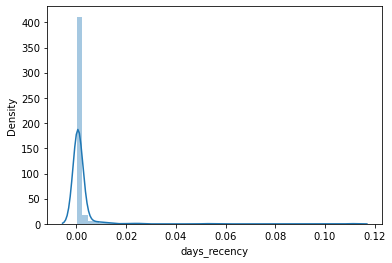
\includegraphics[width=0.4\linewidth]{images/recency_skewed.png}
		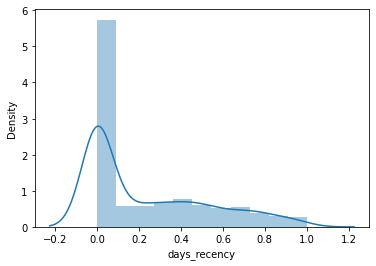
\includegraphics[width=0.4\linewidth]{images/recency_fixed.png} \\
	\end{tabular}
	\caption{left - skewness in recency, right - skewness made better}
	\label{fig:recency_skewness_before_after_fix}
\end{figure}

For each 3 predictions, we perform the following operations:
\begin{enumerate}
    \item We train our model on the \textbf{entire training data} and test on NULL test data.
    \item We compare the distribution of values computed in the previous step with that of the NON-NULL test data
\end{enumerate}

\subsection{Methodology - Deriving Biological Age}
We split the dataset into train and test using \textit{DEATH [d from CT]} column. The data item with non-empty value will go into training data, and rest will be used to check the effectiveness of the methodology. Based on this, we split the original dataset of size 9223 into 549 training items and 8674 test items.

We made few intuitive assumptions:
\begin{enumerate}
    \item People die when they hit biological age 100. Healthy people can slowdown the bio age and that is how some humans live more than 100 chronological age. This gives us \textit{max\_bio\_age\_in\_days} = 36500
    \item Higher the \textit{DEATH[d from CT]}, higher the patient has \textit{ bio\_days\_left} to live
\end{enumerate}

Based on this assumption, we define the biological age for training data as the function of \textit{bio\_days\_left}.

\[ bio\_age = max\_bio\_age\_in\_days - bio\_days\_left  \]

\[ bio\_age\_left = A + C*(1-\exp^{-k*x}) \]

Here, \textit{bio\_days\_left} follows exponential decay 
function(increasing) form as shown in Fig - \ref{fig:exp_decay}

\begin{figure}[H]
\centering
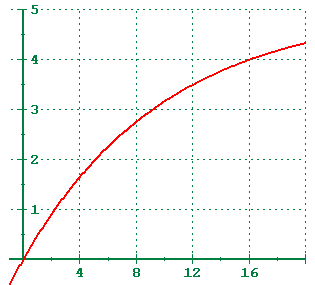
\includegraphics[width=0.3\textwidth]{images/exp_fn.png}
\caption{Example of a exponential decay increasing form plot}
\label{fig:exp_decay}
\end{figure}


We calculate \textit{bio\_days\_left} for training data, and then apply 2 the following 2 algorithms
\begin{enumerate}
    \item Linear Regression
    \item {XGBoost}
\end{enumerate}




\section{Results}

\subsection{Predicting Clinical Outcomes}
For both the approaches mentioned in \textbf{Section 4} we executed 3 machine learning algorithm mentioned in \textbf{Secion 3}.

For approach-1 and \textit{death}, we got the RMSE comparison results using only CT and CT + Clinical data as described in Table \ref{tab:death_approach_1}. XGBoost performed better than its counterparts with both CT and CT + Clinical Data and exhibited the lowest RMSE. 
\begin{table}[H]
\centering
\begin{tabular}{|l|c|l|}
\hline
\textbf{Model}           & \textbf{RMSE (only CT)} & \textbf{RMSE (CT + Clinical)} \\ \hline
Linear Regression        & 1351.75                 & 1324.57                       \\ \hline
Support Vector Regressor & 1410.32                 & 1381.12                       \\ \hline
XGBoost                  & \textbf{1331.59}                 & \textbf{1314.85}                       \\ \hline
\end{tabular}
\caption{Predicting Death Approach-1:Model Comparison}
\label{tab:death_approach_1}
\end{table}

\begin{figure}[H]
	\def\imgwidth{0.5\linewidth}
% 	\setlength\tabcolsep{2pt}
	\centering
	\begin{tabular}{ccc}
		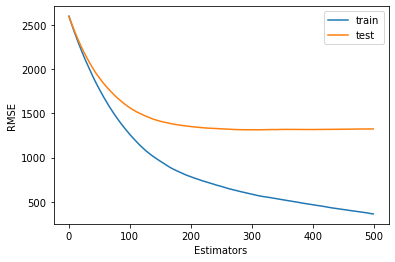
\includegraphics[width=0.3\linewidth]{images/death/a_1_comp_rmse.png} &
		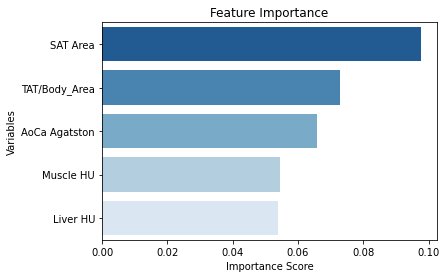
\includegraphics[width=0.3\linewidth]{images/death/a_1_comp_feat_imp.png} &
		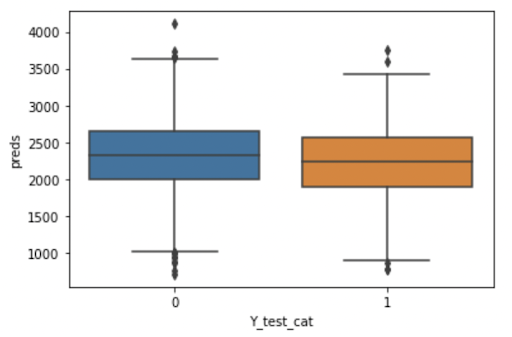
\includegraphics[width=0.3\linewidth]{images/death/a_1_comp_w_test.png} \\
	\end{tabular}
	\caption{XGBoost - Predicting death without recency(approach-1). left = decreasing RMSE with number of iterations, center = feature importance, right = distribution comparison with test-data}
	\label{fig:death_results_a_1}
\end{figure}



For approach-2 and \textit{death}, we got the RMSE comparison results using only CT and CT + Clinical data as described in Table \ref{tab:death_approach_2}. Again, XGBoost performed better than its counterparts with both CT and CT + Clinical Data and exhibited the lowest RMSE. 
\begin{table}[H]
\centering
\begin{tabular}{|l|c|l|}
\hline
\textbf{Model}           & \textbf{RMSE (only CT)} & \textbf{RMSE (CT + Clinical)} \\ \hline
Linear Regression        & 0.235                   & 0.204 (+13.1\%)               \\ \hline
Support Vector Regressor & 0.235                   & 0.243 (-3.4\%)                \\ \hline
XGBoost                  & \textbf{0.232}                   & \textbf{0.212 (+8.6\%)}                \\ \hline
\end{tabular}
\caption{Predicting Death Approach-2:Model Comparison}
\label{tab:death_approach_2}
\end{table}

\begin{figure}[H]
	\def\imgwidth{0.5\linewidth}
% 	\setlength\tabcolsep{2pt}
	\centering
	\begin{tabular}{ccc}
		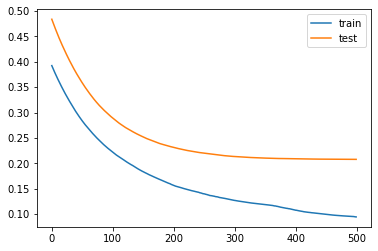
\includegraphics[width=0.3\linewidth]{images/death/a_2_comp_rmse.png} &
		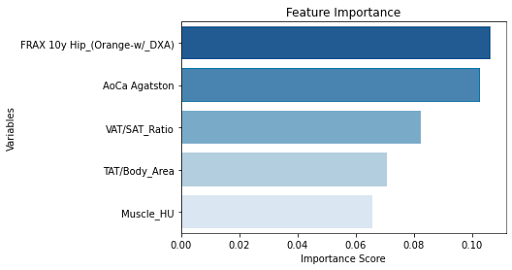
\includegraphics[width=0.3\linewidth]{images/death/a_2_comp_feat_imp.png} &
		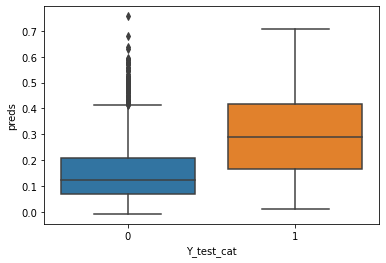
\includegraphics[width=0.3\linewidth]{images/death/a_2_comp_w_test.png} \\
	\end{tabular}
	\caption{XGBoost - Predicting death with recency(approach-2). left = decreasing RMSE with number of iterations, center = feature importance, right = distribution comparison with test-data}
	\label{fig:death_results_a_2}
\end{figure}

We compared the results from both the approaches with the distribution of death, and found out that distribution in approach-1 result is almost same as test-data. However, with approach-2, it is slightly higher(lower because recency is inverse of days). Hence, approach-2 is better.
The approach-1 output SAT Area, TAT/Body Area, AoCa Agatston, Muscle HU, Liver HU as the important features. On the other hand, the approach-2 considers FRAX, AoCa Agatston, VAT/SAT Ratio, TAT/Body Area, Muscle HU. Considering both the approaches, it seems that \textit{AoCa Agatston, TAT/Body Area, Muscle HU} are important features.

\begin{figure}[H]
	\def\imgwidth{0.5\linewidth}
% 	\setlength\tabcolsep{2pt}
	\centering
	\begin{tabular}{cc}
		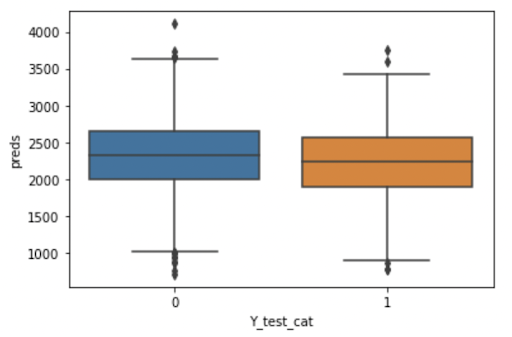
\includegraphics[width=0.4\linewidth]{images/death/a_1_comp_w_test.png} &
		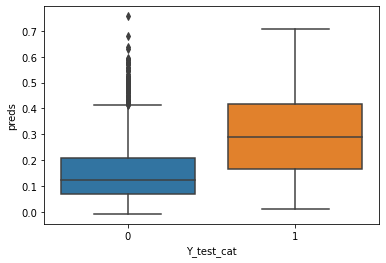
\includegraphics[width=0.4\linewidth]{images/death/a_2_comp_w_test.png} \\
	\end{tabular}
	\caption{Comparison of both the approaches with test data on death distribution. left=approach-1, right=approach-2}
	\label{fig:death_results_dist_comp_with_test_data}
\end{figure}

We continued the same experiments with other clinical outcomes, and found out that \textit{recency} approach is effective in the given dataset.

For approach-2 and \textit{diabetes}, we got the RMSE comparison results using only CT and CT + Clinical data as described in Table \ref{tab:diabetes_approach_2}. Linear Regression performed better than its counterparts with both CT and CT + Clinical Data and exhibited the lowest RMSE. 
\begin{table}[H]
\centering
\begin{tabular}{|l|c|l|}
\hline
\textbf{Model}           & \textbf{RMSE (only CT)} & \textbf{RMSE (CT + Clinical)} \\ \hline
Linear Regression        & \textbf{0.248}                   & \textbf{0.243 (-2\%)}         \\ \hline
Support Vector Regressor & 0.253                   & 0.258 (+1.9\%)                \\ \hline
XGBoost                  & 0.257                   & 0.251 (-2.3\%)                \\ \hline
\end{tabular}
\caption{Predicting Diabetes Approach-2:Model Comparison}
\label{tab:diabetes_approach_2}
\end{table}


For approach-2 and \textit{heart attack}, we got the RMSE comparison results using only CT and CT + Clinical data as described in Table \ref{tab:diabetes_approach_2}. Linear Regression and XGBoost both performed better than Support Vector Regressor with both CT and CT + Clinical Data and exhibited the great improvements. 
\begin{table}[H]
\centering
\begin{tabular}{|l|c|l|}
\hline
\textbf{Model}           & \textbf{RMSE (only CT)} & \textbf{RMSE (CT + Clinical)} \\ \hline
Linear Regression        & 0.223                   & \textbf{0.221 (-0.8\%)}       \\ \hline
Support Vector Regressor & 0.243                   & 0.241 (+0.8\%)                \\ \hline
XGBoost                  & 0.245                   & \textbf{0.230 (-6.1\%)}       \\ \hline
\end{tabular}
\caption{Predicting Heart Attack Approach-2:Model Comparison}
\label{tab:heart_attack_approach_2}
\end{table}
% \input{results/death}
% \input{results/diabetes}
% \input{results/heart_attack}

\subsection{Deriving a Biological Age}
We executed the approach mentioned in the \textbf{Section - 4} on both \textit{Linear Regression} and \textit{XGBoost} algorithms.
As shown in the Fig - \ref{fig:bio_age_results_comp_with_test_data} Linear Regression performs worse and is concentrated around somewhere between 75-85 for most test samples. However, XGBoost shows Gaussian distribution and scattered nicely, which shows better fit.

\begin{figure}[H]
	\def\imgwidth{0.5\linewidth}
	\centering
	\begin{tabular}{cc}
		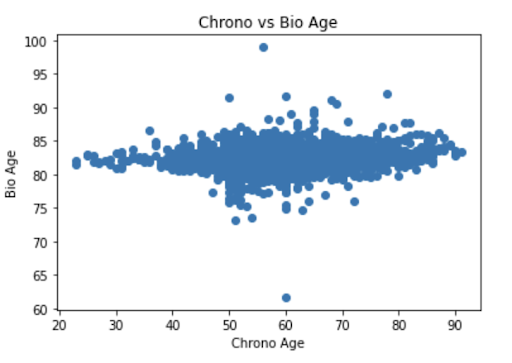
\includegraphics[width=0.4\linewidth]{images/bio_age/bio_lr.png} &
		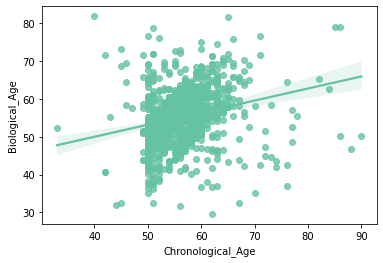
\includegraphics[width=0.4\linewidth]{images/bio_age/bio_xgboost.png} \\
	\end{tabular}
	\caption{Biological Age: comparison of both the algorithm on test-data left=Linear Regression, right=XGBoost}
	\label{fig:bio_age_results_comp_with_test_data}
\end{figure}

Next, we show in Fig - \ref{fig:bio_age_results_body}  correlation of features such as muscle mass, muscle area and calcification with Biological age. Muscle Mass and Muscle Area are decreasing as Biological age increases. Calcification is increasing as Biological age increases.

\begin{figure}[H]
	\def\imgwidth{0.5\linewidth}
% 	\setlength\tabcolsep{2pt}
	\centering
	\begin{tabular}{ccc}
		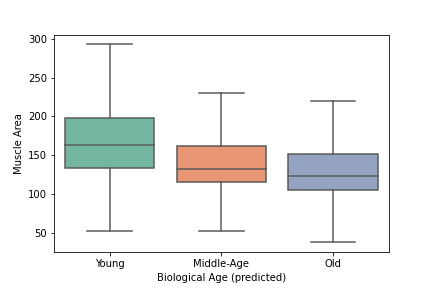
\includegraphics[width=0.3\linewidth]{images/bio_age/bio_muscle_area.png} &
		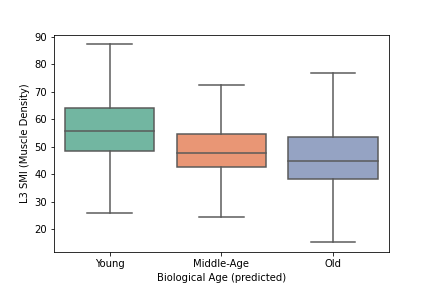
\includegraphics[width=0.3\linewidth]{images/bio_age/bio_muscle_mass.png} &
		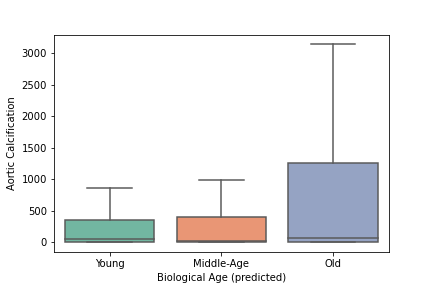
\includegraphics[width=0.3\linewidth]{images/bio_age/bio_calci.png} \\
	\end{tabular}
	\caption{Effect on body as bio age is increasing. left = decreasing muscle area, center = decreasing muscle mass, right = increasing calcification}
	\label{fig:bio_age_results_body}
\end{figure}
\section{Conclusion}
We shown in the project that it CT + Clinical data is better at predicting critical clinical outcomes such as \textit{death, diabetes and heart-attack}. Moreover, CT data contains effective biological health-markers that can be used to assess how is patient doing biological health-wise. Although limited, for this dataset, XGBoost seems to be performing well in most cases.

One can find the entire project on GitHub \cite{github}
\section{Aknowledgement}

We would like to thank Prof Danile Pimental (Department of Bio Statistics, UW-Madison) and Perry Pickhardt (Department of Radiology, UW-Madison) for their constant support and guidance in our endeavour. It would not be possible without their encouragement and constant quest of improvisation.

% \bibliographystyle{acm}
% \bibliography{references}

\begin{thebibliography}{9}

\bibitem{common_methods_of_biological_age_estimation}
Jia L, Zhang W, Chen X. Common methods of biological age estimation. Clin Interv Aging. 2017;12:759-772. Published 2017 May 11. doi:10.2147/CIA.S134921

\bibitem{60_new_50}
Levine ME, Crimmins EM. Is 60 the New 50? Examining Changes in Biological Age Over the Past Two Decades. Demography. 2018;55(2):387-402. doi:10.1007/s13524-017-0644-5

\bibitem{bio_using_PCA}
Jia L, Zhang W, Jia R, Zhang H, Chen X. Construction Formula of Biological Age Using the Principal Component Analysis. Biomed Res Int. 2016;2016:4697017. doi:10.1155/2016/4697017

\bibitem{FAT}
Shuster A, Patlas M, Pinthus JH, Mourtzakis M. The clinical importance of visceral adiposity: a critical review of methods for visceral adipose tissue analysis. Br J Radiol. 2012;85(1009):1-10. doi:10.1259/bjr/38447238

\bibitem{BMD}
Yaprak, G., Gemici, C., Seseogullari, O. O., Karabag, I. S.; Cini, N. (2020). CT derived Hounsfield Unit: An easy way to determine osteoporosis and radiation related fracture risk in irradiated patients. Frontiers in Oncology, 10. https://doi.org/10.3389/fonc.2020.00742

\bibitem{Liver HU}
Hamer, O. W., Aguirre, D. A., Casola, G., Lavine, J. E., Woenckhaus, M.; Sirlin, C. B. (2006). Fatty liver: Imaging patterns and pitfalls. RadioGraphics, 26(6), 1637–1653. https://doi.org/10.1148/rg.266065004 

\bibitem{AoCa}
Mayo Foundation for Medical Education and Research. (2021, July 23). Heart scan (coronary calcium scan). Mayo Clinic. Retrieved May 12, 2022, from https://www.mayoclinic.org/tests-procedures/heart-scan/about/pac-20384686

\bibitem{imputing}
Tackling missing value in dataset. Analytics Vidhya. (2021, November 12). Retrieved May 12, 2022, from https://www.analyticsvidhya.com/blog/2021/10/handling-missing-value

\bibitem{github}
https://github.com/SahuH/CS760-project

\end{thebibliography}

\end{document} 
\endinput
































